
\documentclass[11pt]{article}
\usepackage[utf8]{inputenc}
\usepackage[T1]{fontenc}
\usepackage{lmodern}
\usepackage{amsmath, amssymb, amsthm}
\usepackage{graphicx}
\usepackage{hyperref}
\usepackage{geometry}
\geometry{margin=1in}

\title{Lemniscata de Penin ($\infty\!\!\diagup$): Evolução Infinita sob Trilhos}
\author{Daniel Penin}
\date{2025}

\begin{document}
\maketitle

\begin{abstract}
Propomos a \textbf{Lemniscata de Penin}, um operador de evolução infinita segura, formalizado por
\[ P = \infty\!\!\diagup(E + N - iN), \qquad iN = (1 - I)N,\; I\in[0,1]. \]
Ao incorporar a integridade $I$ no núcleo, o operador $\infty\!\!\diagup$ atua como um guardião que
permite progresso ilimitado sob trilhos, evitando colapsos. Apresentamos a formulação, um
modelo programático mínimo e resultados de simulação comparando com um baseline sem trilhos.
\end{abstract}

\section{Introdução}
A Equação de Turing (ET$\Omega$) consolidou a ideia de evolução guiada, mas dependia de parâmetros e verificações externas.
A Lemniscata de Penin sintetiza o princípio em um operador único $\infty\!\!\diagup$, substituindo ajustes manuais por integridade embutida.

\section{Definição Formal}
Definimos
\[ P = \infty\!\!\diagup(E + N - iN), \qquad iN = (1 - I)N, \]
onde $E$ representa eficiência útil, $N$ novidade informativa e $I$ a integridade da proposta.
O termo $iN$ mede a fração inadmissível de $N$ e é automaticamente suprimido pelo operador.

\section{Formalização Algorítmica}
Um esboço em Python do operador é dado por:
\begin{verbatim}
class LemniscataPenin:
    def __call__(self, E, N, I):
        iN = (1 - I) * max(0, N)
        P  = E + N - iN
        return max(E, P)
\end{verbatim}
Este núcleo define o \emph{infinito sob trilhos}: evolução contínua sem regressões quando $I$ decai.

\section{Simulação}
Utilizamos uma simulação com 300 iterações. Em cada passo, propõe-se uma novidade $N$ e estima-se um risco
proporcional a $N$, definindo $I=1-\text{risco}$. Comparamos:
(i) sistema com $\infty\!\!\diagup$; (ii) baseline sem trilhos (aceita tudo).

\subsection{Resultados}
A Figura~\ref{fig:efficiency} ilustra a evolução da eficiência. O operador $\infty\!\!\diagup$ mantém
crescimento estável; o baseline sofre instabilidades sob alto risco.
\begin{figure}[h]
  \centering
  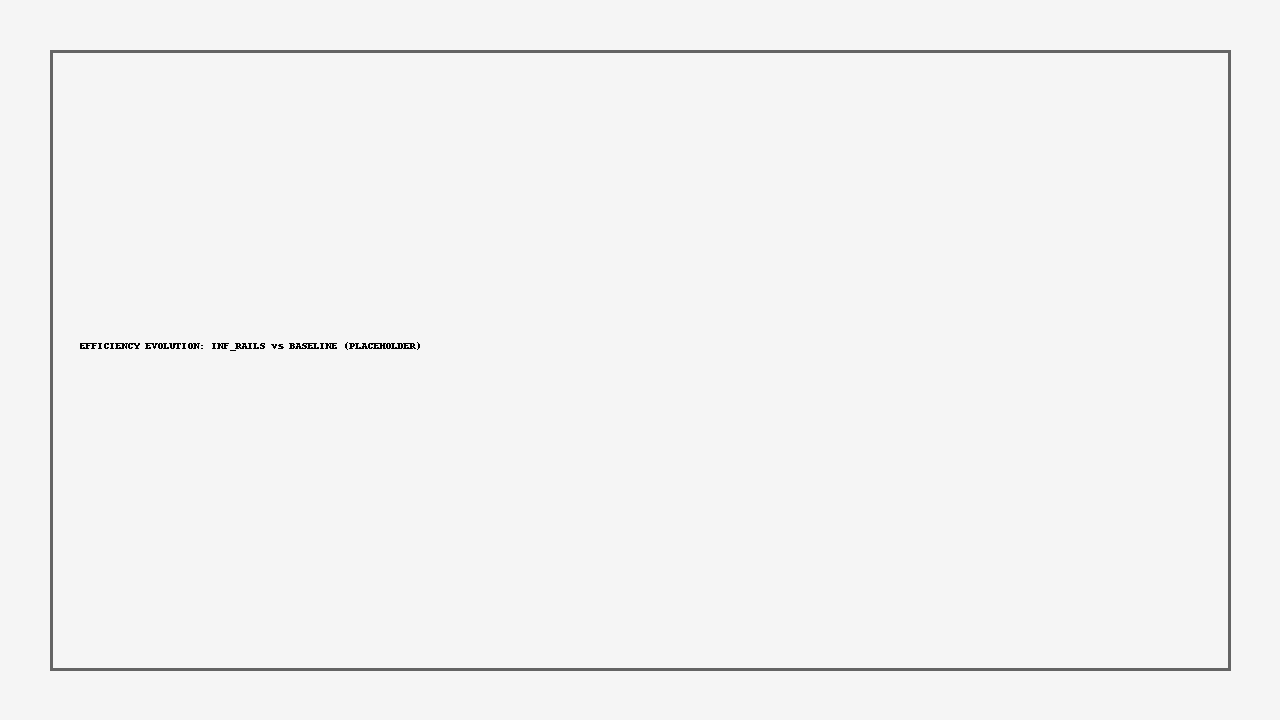
\includegraphics[width=0.85\linewidth]{figures/efficiency_placeholder.png}
  \caption{Evolução da eficiência: $\infty\!\!\diagup$ vs. sem trilhos (placeholder).}
  \label{fig:efficiency}
\end{figure}

\section{Discussão}
A Lemniscata de Penin combina simplicidade e universalidade (análoga a fórmulas canônicas, como $E=mc^2$),
abrindo caminho a aplicações em IA evolutiva segura, sistemas multiagente e integrações quânticas.

\section{Conclusão}
O operador $\infty\!\!\diagup$ propicia evolução infinita sob trilhos, eliminando platôs e colapsos sem
hiperparâmetros frágeis. Sugerimos sua adoção como paradigma padrão para evolução segura de inteligência.

\bibliographystyle{plain}
\bibliography{lemniscata}

\end{document}
